\chapter{Leviticus 10}

\begin{figure}
  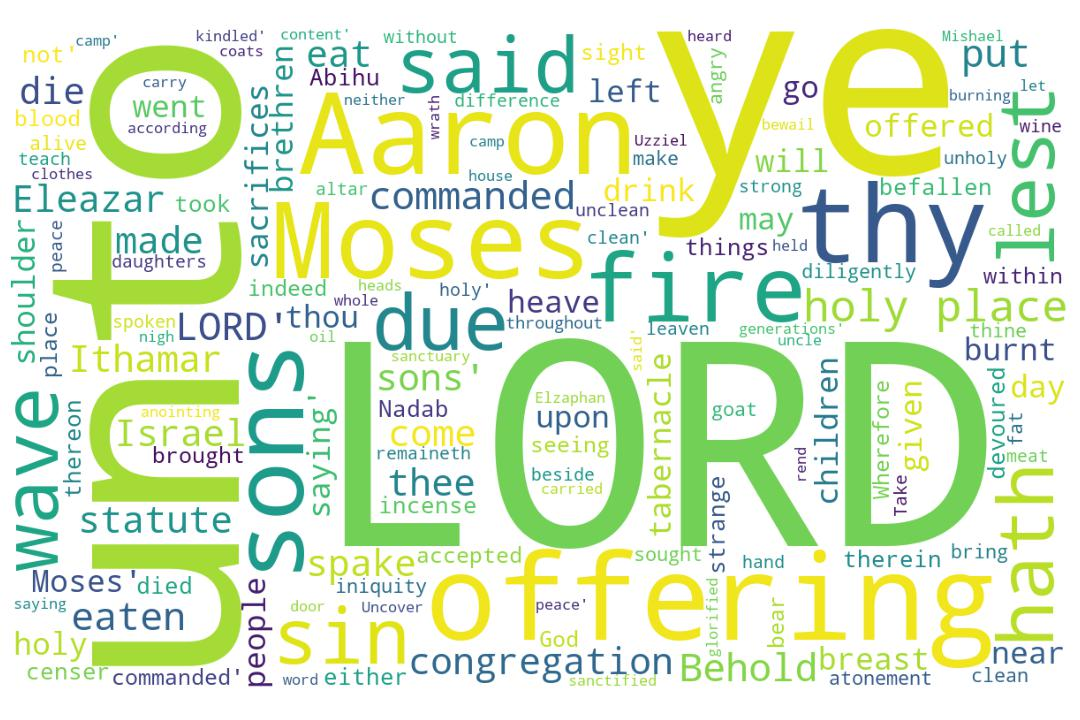
\includegraphics[width=\linewidth]{03OT-Leviticus/Leviticus10-WordCloud.jpg}
  \caption{Leviticus 10 Word Cloud}
  \label{fig:Leviticus 10 word Cloud}
\end{figure}

\marginpar{\scriptsize \centering \fcolorbox{bone}{lime}{\textbf{STRANGE FIRE}}\\ (Leviticus 10:1--20) 
\begin{compactenum}[I.][8]
	\item The \textbf{Censers} \index[scripture]{Leviticus!Lev 10:01}(Lev 10:1)
	\item The \textbf{Corruption} \index[scripture]{Leviticus!Lev 10:02}(Lev 10:2)
	\item The \textbf{Consumption} \index[scripture]{Leviticus!Lev 10:02}(Lev 10:2)
	\item The \textbf{Corpses}  \index[scripture]{Leviticus!Lev 10:04}(Lev 10:4)
	\item The \textbf{Carrying} Away \index[scripture]{Leviticus!Lev 10:05}(Lev 10:5) cf \index[scripture]{Acts!Acts 05:09}(Acts 5:9)
	\item The \textbf{Congregation}  \index[scripture]{Leviticus!Lev 10:07}\index[scripture]{Leviticus!Lev 10:09}\index[scripture]{Leviticus!Lev 10:17}(Lev 10:7, 9, 17) (which undoubtedly sought an explanation)
	\item The \textbf{Correction}  \index[scripture]{Leviticus!Lev 10:09--10}(Lev 10:9--10) (establishing the distinction between holy and unholy)
\end{compactenum} }

%%%%%%%%%%%%%%%%%%%%%%%%%%%
%%%%%%%%%%%%%%%%%%%%%%%%%%%
\footnote{\textcolor[cmyk]{0.99998,1,0,0}{\hyperlink{TOC}{Return to end of Table of Contents.}}}\footnote{\href{https://audiobible.com/bible/leviticus_10.html}{\textcolor[cmyk]{0.99998,1,0,0}{Leviticus 10 Audio}}}\textcolor[cmyk]{0.99998,1,0,0}{And Nadab and Abihu, the sons of Aaron, took either of them his \fcolorbox{bone}{lime}{censer}, and put fire therein, and put incense thereon, and offered strange fire before the LORD, which he commanded them not.}
[2] \textcolor[cmyk]{0.99998,1,0,0}{And there went out fire from the LORD, and \fcolorbox{bone}{lime}{devoured} them, and \fcolorbox{bone}{lime}{they died} before the LORD.}
[3] \textcolor[cmyk]{0.99998,1,0,0}{Then Moses said unto Aaron, This \emph{is} \emph{it} that the LORD spake, saying, I will be sanctified in them that come nigh me, and before all the people I will be glorified. And Aaron held his peace.}
[4] \textcolor[cmyk]{0.99998,1,0,0}{And Moses called Mishael and Elzaphan, the sons of Uzziel the uncle of Aaron, and said unto them, Come near, \fcolorbox{bone}{lime}{carry your brethren} from before the sanctuary out of the camp.}
[5] \textcolor[cmyk]{0.99998,1,0,0}{So they went near, and \fcolorbox{bone}{lime}{carried} them in their coats out of the camp; as Moses had said.}
[6] \textcolor[cmyk]{0.99998,1,0,0}{And Moses said unto Aaron, and unto Eleazar and unto Ithamar, his sons, Uncover not your heads, neither rend your clothes; lest ye die, and lest wrath come upon all the people: but let your brethren, the whole house of Israel, bewail the burning which the LORD hath kindled.}
[7] \textcolor[cmyk]{0.99998,1,0,0}{And ye shall not go out from the door of the tabernacle of the \fcolorbox{bone}{lime}{congregation}, lest ye die: for the anointing oil of the LORD \emph{is} upon you. And they did according to the word of Moses.}\\
\\
\P \textcolor[cmyk]{0.99998,1,0,0}{And the LORD spake unto Aaron, saying,}
[9] \textcolor[cmyk]{0.99998,1,0,0}{Do not drink wine nor strong drink, thou, nor thy sons with thee, when ye go into the tabernacle of the congregation, lest ye die: \emph{it} \emph{shall} \emph{be} a statute for ever throughout your generations:}
[10] \textcolor[cmyk]{0.99998,1,0,0}{And that ye may put \fcolorbox{bone}{lime}{difference} between holy and unholy, and between unclean and clean;}
[11] \textcolor[cmyk]{0.99998,1,0,0}{And that ye may teach the children of Israel all the statutes which the LORD hath spoken unto them by the hand of Moses.}\\
\\
\P \textcolor[cmyk]{0.99998,1,0,0}{And Moses spake unto Aaron, and unto Eleazar and unto Ithamar, his sons that were left, Take the meat offering that remaineth of the offerings of the LORD made by fire, and eat it without leaven beside the altar: for it \emph{is} most holy:}
[13] \textcolor[cmyk]{0.99998,1,0,0}{And ye shall eat it in the holy place, because it \emph{is} thy due, and thy sons' due, of the sacrifices of the LORD made by fire: for so I am commanded.}
[14] \textcolor[cmyk]{0.99998,1,0,0}{And the wave breast and heave shoulder shall ye eat in a clean place; thou, and thy sons, and thy daughters with thee: for \emph{they} \emph{be} thy due, and thy sons' due, \emph{which} are given out of the sacrifices of peace offerings of the children of Israel.}
[15] \textcolor[cmyk]{0.99998,1,0,0}{The heave shoulder and the wave breast shall they bring with the offerings made by fire of the fat, to wave \emph{it} \emph{for} a wave offering before the LORD; and it shall be thine, and thy sons' with thee, by a statute for ever; as the LORD hath commanded.}\\
\\
\P \textcolor[cmyk]{0.99998,1,0,0}{And Moses diligently sought the goat of the sin offering, and, behold, it was burnt: and he was angry with Eleazar and Ithamar, the sons of Aaron \emph{which} \emph{were} left \emph{alive}, saying,}
[17] \textcolor[cmyk]{0.99998,1,0,0}{Wherefore have ye not eaten the sin offering in the holy place, seeing it \emph{is} most holy, and \emph{God} hath given it you to bear the iniquity of the congregation, to make atonement for them before the LORD?}
[18] \textcolor[cmyk]{0.99998,1,0,0}{Behold, the blood of it was not brought in within the holy \emph{place}: ye should indeed have eaten it in the holy \emph{place}, as I commanded.}
[19] \textcolor[cmyk]{0.99998,1,0,0}{And Aaron said unto Moses, Behold, this day have they offered their sin offering and their burnt offering before the LORD; and such things have befallen me: and \emph{if} I had eaten the sin offering to day, should it have been accepted in the sight of the LORD?}
[20] \textcolor[cmyk]{0.99998,1,0,0}{And when Moses heard \emph{that}, he was content.}